%% ============================================================
%% GHG Quantification — Thailand Rice CH4 Emissions (SHORT VERSION)
%% IPEN6100F Final Project | Template: olplainarticle
%% Compile: pdflatex → bibtex → pdflatex → pdflatex
%% ============================================================

\documentclass[fleqn,10pt]{olplainarticle}

\usepackage{newtxtext,newtxmath}
\usepackage{setspace}
\usepackage{microtype}
\usepackage{booktabs}
\usepackage{float}
\usepackage{placeins}
\usepackage{amsmath}
\usepackage{array}

\title{Price Policy as a Driver of Agricultural Methane: Evidence from
       Thailand's Rice Sector, 1961--2024}

\author[1]{Sirawit Tangchiitwatthanakon}
\affil[1]{The Hong Kong University of Science and Technology (Guangzhou), Guangzhou, China}

\keywords{methane emissions; paddy rice cultivation; greenhouse gas inventory;
          IPCC Tier~1 methodology; Thailand; agricultural price support;
          Nationally Determined Contribution}

\begin{abstract}
Rice paddies are a major source of methane (CH\textsubscript{4}), a greenhouse
gas with a 100-year global warming potential (GWP\textsubscript{100}) of 28.
Thailand, one of the world's top rice exporters, cultivates approximately
11~million hectares annually, making accurate CH\textsubscript{4} estimation
essential for national climate reporting.
This study applies IPCC 2006 Tier~1 to estimate national rice CH\textsubscript{4}
emissions from 1961 to 2024 and to examine how the \textit{structural design}
of price-support programmes determines their emission impact.
National emissions averaged \textbf{1,420~Gg~CH\textsubscript{4}~yr\textsuperscript{-1}}
(39.8~Mt~CO\textsubscript{2}e), peaking at 1,884~Gg in 2012.
The 2011--2014 Rice Pledging Scheme, an unlimited price guarantee at 40--50\%
above market, added an estimated 988,000~ha beyond the price effect alone
($p < 0.001$).
A counterfactual estimate shows that a per-household area cap applied from 2011
would have avoided \textbf{606~Gg~CH\textsubscript{4}} (17.0~Mt~CO\textsubscript{2}e)
over four years, more than five times the annual mitigation potential of full
AWD adoption.
Emission intensity fell 44\% as yields improved, yet absolute emissions rose
84\%: yield gains raised farming profitability and attracted area expansion,
illustrating that yield improvement alone does not reduce absolute CH\textsubscript{4}.
These findings indicate that Thailand's NDC agriculture targets are more
sensitive to price-support programme design than to yield improvement or
field-level mitigation technology alone.
\end{abstract}

\begin{document}
\onehalfspacing
\flushbottom
\maketitle
\thispagestyle{empty}

% =============================================================
\section*{Introduction}
% =============================================================

Thailand is one of the world's top rice exporters \citep{faostat2026},
devoting over 11~million hectares to paddy cultivation each year.
These flooded fields produce CH\textsubscript{4}, a greenhouse gas with a
GWP\textsubscript{100} of 28 that has contributed approximately 20\% of
human-caused radiative forcing since pre-industrial times \citep{myhre2013}.
Flooded rice paddies alone emit 25--60~Tg~CH\textsubscript{4}~yr\textsuperscript{-1},
roughly 10--12\% of the global CH\textsubscript{4} budget
\citep{neue1993, yan2009}.
In flooded fields, microbes break down organic matter without oxygen and release
CH\textsubscript{4}; the gas escapes mainly through hollow channels in the rice
plant's stem \citep{neue1993}.
Because emission rates scale directly with flooded area and growing period
\citep{ipcc2006}, any expansion of rice cultivation directly increases emissions.

Despite this, the link between rice price policy and CH\textsubscript{4}
emissions has received limited scientific attention.
This study has two objectives: (1)~to quantify Thailand's national rice
CH\textsubscript{4} trend from 1961 to 2024; and (2)~to examine how farm-gate
price policy drives year-to-year emission changes.

% =============================================================
\section*{Data and Methodology}
% =============================================================

\subsection*{Data}

Annual rice harvested area (1961--2024) was obtained from FAOSTAT
\citep{faostat2026} (element code~5312).
Monthly farm-gate paddy prices (THB~tonne\textsuperscript{-1}, 15\% moisture
content, 2007--2024) were obtained from Thailand's Office of Agricultural
Economics (OAE) \citep{oae2024} and converted to annual averages.

\subsection*{Emission calculation}

CH\textsubscript{4} emissions follow IPCC 2006 Guidelines, Vol.~4, Ch.~5
\citep{ipcc2006}:

\begin{equation}
  \text{CH}_{4,i} = \text{EF}_i \times A_i \times 10^{-6}
  \label{eq:ch4}
\end{equation}

\noindent where $\text{CH}_{4,i}$ is annual emission (Gg~yr\textsuperscript{-1}),
$A_i$ is harvested area (ha), and the seasonal emission factor is:

\begin{equation}
  \text{EF}_i = \text{EF}_c \times \text{SF}_{w} \times \text{SF}_{p}
               \times \text{SF}_{o} \times t_{p}
  \label{eq:ef}
\end{equation}

Tier~1 default scaling factors ($\text{SF}_w = \text{SF}_p = \text{SF}_o = 1.0$)
yield emission factors of 153.4~kg~ha\textsuperscript{-1} for the main season
(118~days) and 144.3~kg~ha\textsuperscript{-1} for the dry season (111~days)
\citep{buddhaboon2011}.
CO\textsubscript{2}-equivalent emissions use GWP\textsubscript{100} = 28
\citep{myhre2013}.
Because EF is constant under Tier~1, CH\textsubscript{4} is an exact linear
function of harvested area, meaning the price--CH\textsubscript{4} correlation
is mathematically identical to the price--area correlation.

\subsection*{Statistical analysis}

Pearson correlation tested the relationship between farm-gate price and
harvested area for 2007--2024 ($n = 18$).
A multivariate OLS regression included a binary policy dummy
($D_t = 1$ for 2011--2014 Pledging Scheme years):

\begin{equation}
  A_t = \beta_0 + \beta_1 P_t + \beta_2 D_t + \varepsilon_t
  \label{eq:dummy}
\end{equation}

Newey--West HAC standard errors \citep{neweywest1987} correct for serial
dependence in the annual time series.

% =============================================================
\section*{Results and Discussion}
% =============================================================

\subsection*{National emission trend, 1961--2024}

Thailand's mean annual rice CH\textsubscript{4} emission was
\textbf{1,420~Gg~CH\textsubscript{4}~yr\textsuperscript{-1}}
(39.8~Mt~CO\textsubscript{2}e; Table~\ref{tab:national}).
Emissions rose significantly at +12.0~Gg~yr\textsuperscript{-1}
($R^2 = 0.830$, $p < 0.001$) from 939~Gg in 1961 to a peak of
\textbf{1,884~Gg in 2012}, before declining to 1,726~Gg (48.3~Mt~CO\textsubscript{2}e)
in 2024, approximately 13\% of Thailand's total national GHG emissions
\citep{tgo2022}.
Long-run growth reflects government irrigation investment and Green Revolution
variety adoption in the 1960s--1980s, followed by export-driven expansion
from the 1990s onward.
The 2012 peak stands apart, driven by a price-support policy rather than
structural forces (discussed below).

\begin{table}[!htbp]
\centering
\caption{Summary statistics of national rice CH\textsubscript{4} emissions,
         Thailand, 1961--2024.}
\label{tab:national}
\begin{tabular}{@{}lrl@{}}
\toprule
\textbf{Indicator} & \textbf{Value} & \textbf{Unit} \\
\midrule
Mean CH\textsubscript{4} (1961--2024) & 1,420.0 & Gg~CH\textsubscript{4}~yr\textsuperscript{-1} \\
Minimum CH\textsubscript{4} (1961)    & 938.8   & Gg~CH\textsubscript{4}~yr\textsuperscript{-1} \\
Peak CH\textsubscript{4} (2012)       & 1,883.6 & Gg~CH\textsubscript{4}~yr\textsuperscript{-1} \\
CH\textsubscript{4} in 2024           & 1,725.5 & Gg~CH\textsubscript{4}~yr\textsuperscript{-1} \\
Linear trend                          & +12.0   & Gg~CH\textsubscript{4}~yr\textsuperscript{-1} \\
$R^2$ / $p$-value                     & 0.830 / $<$0.001 & --- \\
Change 1961--2024                     & +83.8   & \% \\
\bottomrule
\end{tabular}
\end{table}

The Northeast region dominates provincial emissions (55\%, 927.0~Gg~yr\textsuperscript{-1}),
driven by its vast rainfed paddy area on the Khorat Plateau.
\textbf{Ubon Ratchathani} is the highest-emitting province
(101.4~Gg~yr\textsuperscript{-1}).
National emission intensity fell from 92.5 to 51.4~kg~CH\textsubscript{4}~t\textsuperscript{-1}
($-$44\%, $R^2 = 0.892$, $p < 0.001$) as nationwide yield growth reduced
the climate cost per tonne of rice, though total emissions still rose 84\%
as area expanded faster than yields improved.

\subsection*{Rice price policy and emission drivers}

Figure~\ref{fig:policy} overlays farm-gate price, harvested area, and
CH\textsubscript{4} from 2007 to 2024.
The co-movement is striking.
The \textbf{Rice Pledging Scheme} (\textit{khrongkan rap chamnam khao};
2011--2014) obliged the government to purchase all paddy at
15,000--20,000~THB~tonne\textsuperscript{-1}, approximately 40--50\% above
world market prices, with \textbf{no quantity cap per household}
\citep{poapongsakorn2014}.
Farmers responded by converting non-rice land to paddy and expanding
double-cropping, pushing harvested area to record levels and CH\textsubscript{4}
to its 64-year peak of 1,884~Gg in 2012.
The scheme cost approximately 984~billion~THB (USD~32~billion) before being
cancelled after the May 2014 military coup; area and emissions contracted
immediately after \citep{poapongsakorn2014, usda2017}.

\begin{figure}[!htbp]
\centering
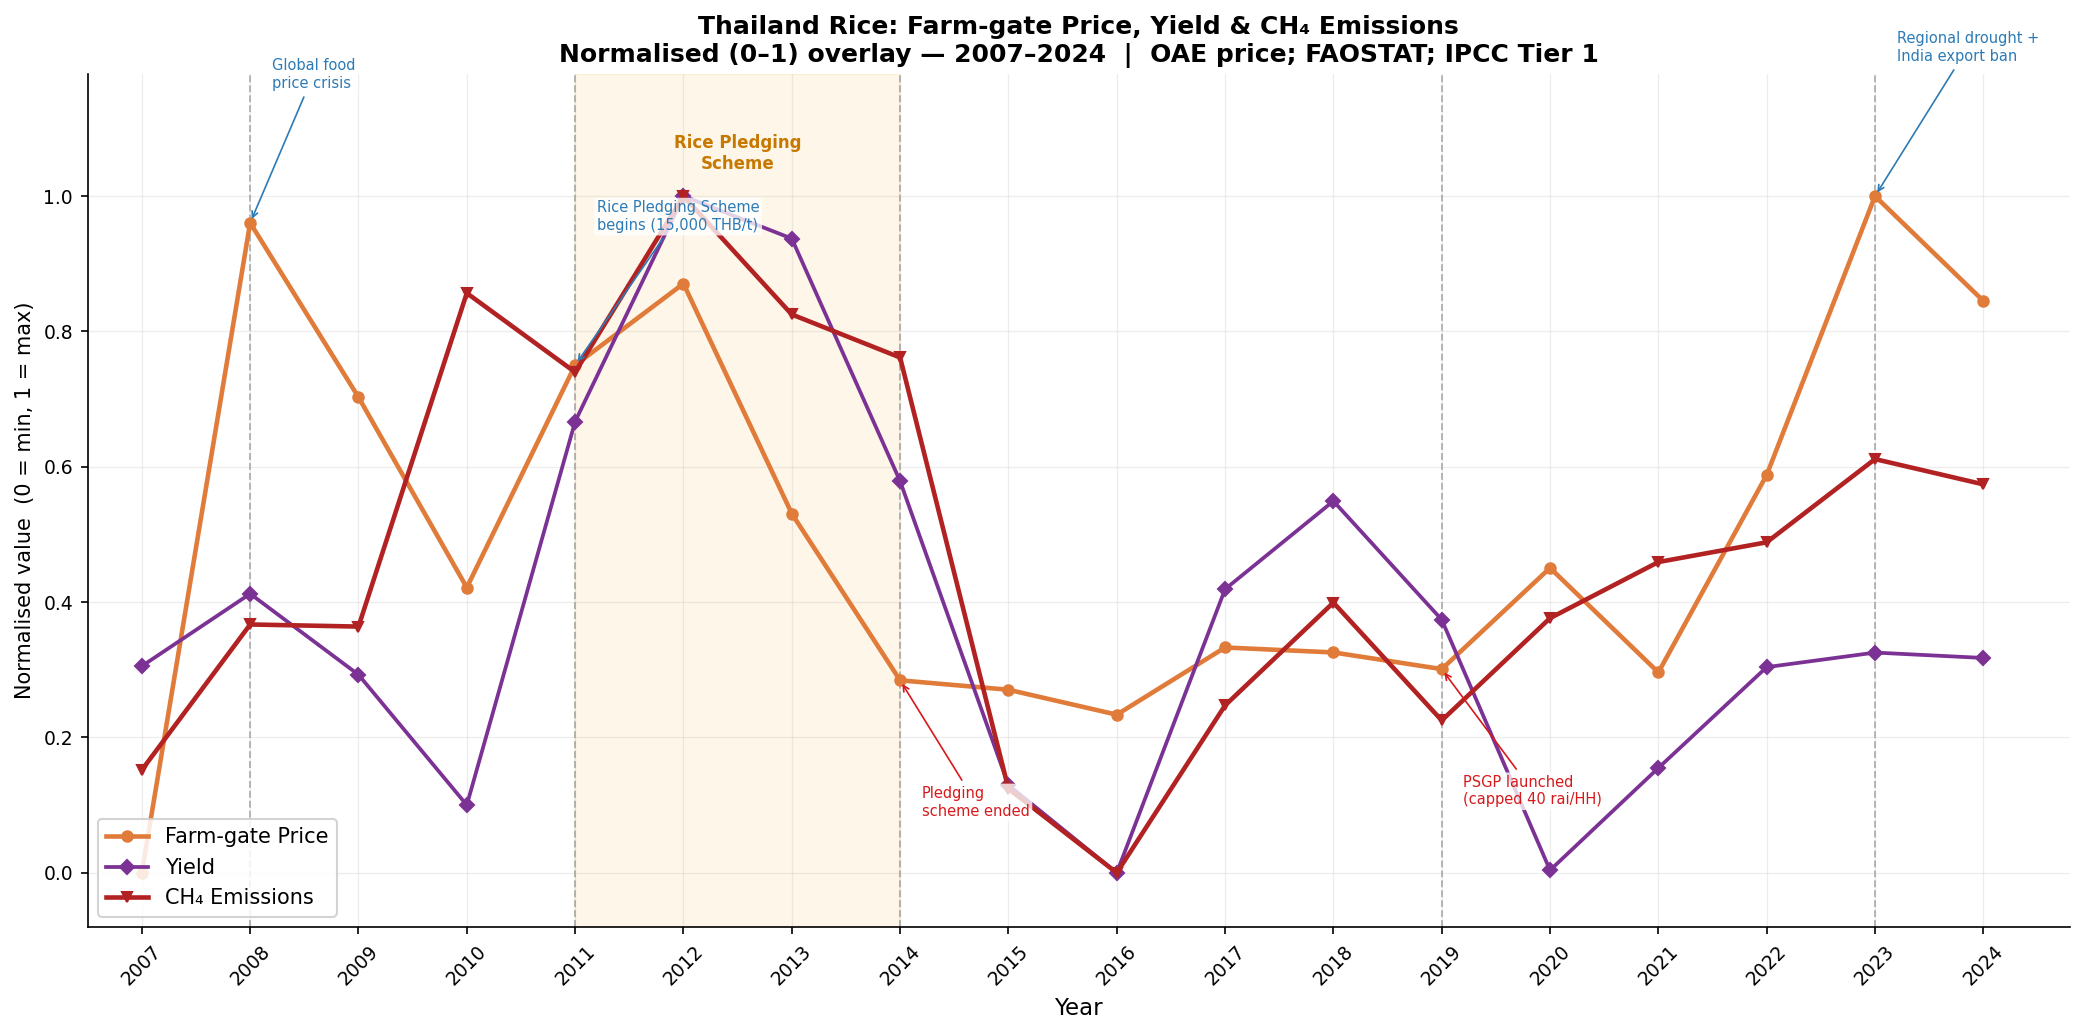
\includegraphics[width=0.96\linewidth]{plot6_policy_timeline.png}
\caption{Thailand rice farm-gate price, harvested area, and CH\textsubscript{4}
         emissions, 2007--2024. Vertical dashed lines mark major policy events.
         Sources: \cite{oae2024}; \cite{faostat2026}; authors' calculation.}
\label{fig:policy}
\end{figure}

Statistical analysis confirms a significant positive link between farm-gate
price and harvested area ($r = 0.505$, $p = 0.033$).
The policy dummy regression (Table~\ref{tab:dummy}) shows the Pledging Scheme
added approximately \textbf{988,000~ha} beyond the price effect alone
($p < 0.001$), equivalent to \textbf{151.6~Gg~CH\textsubscript{4}~yr\textsuperscript{-1}}.
Since 2015, the lighter-touch \textbf{Price Subsidy Guarantee Programme}
(PSGP), capped at 40~rai (6.4~ha) per household, has produced more stable
area and price trajectories, demonstrating that emissions-aware policy design
is achievable without removing farmer income support.

A counterfactual estimate quantifies the emission cost of the design
difference: had the Pledging Scheme imposed the same 40-rai per-household cap
from 2011, the structural excess area ($\hat{\beta}_2 = 988$~kha) would have
been constrained, avoiding an estimated \textbf{606~Gg~CH\textsubscript{4}}
(17.0~Mt~CO\textsubscript{2}e) over the scheme's four-year duration.
This exceeds the annual AWD mitigation potential estimated in this study
(74.6--124.1~Gg~yr\textsuperscript{-1}) by a factor of five to eight per
scheme year, illustrating that programme-design decisions carry greater
emission leverage than field-level mitigation technologies alone.

\begin{table}[!htbp]
\centering
\caption{Regression of national harvested area on price and Pledging Scheme
         dummy, Thailand, 2007--2024 ($n = 18$).
         HAC = Newey--West standard errors \citep{neweywest1987}.}
\label{tab:dummy}
\begin{tabular}{@{}lrrr@{}}
\toprule
 & \textbf{Model 1} & \textbf{Model 2} & \textbf{Model 2 (HAC)} \\
 & \textit{Price only} & \textit{Price + dummy} & \textit{NW SE} \\
\midrule
Intercept & 8{,}490{,}000 ha & 8{,}869{,}000 ha & 8{,}869{,}000 ha \\
Price ($\hat{\beta}_1$, ha/THB~t\textsuperscript{-1}) & 291 & 222 & 222 \\
\quad $p$-value & 0.033 & 0.029 & \textbf{0.005} \\
Pledging dummy ($\hat{\beta}_2$, kha) & --- & $+$988 & $+$988 \\
\quad $p$-value & --- & 0.001 & \textbf{$<$0.001} \\
\midrule
$R^2$ & 0.255 & 0.631 & --- \\
Durbin--Watson & 1.162 & 2.141 & --- \\
\bottomrule
\multicolumn{4}{@{}l@{}}{\footnotesize CH\textsubscript{4} equivalent of $\hat{\beta}_2$: 151.6~Gg~yr\textsuperscript{-1} (EF = 153.4~kg~ha\textsuperscript{-1}, \citealt{buddhaboon2011}).}
\end{tabular}
\end{table}

\subsection*{Limitations}

This study applies Tier~1 uniform emission factors ($\text{SF}_w = 1.0$),
which overestimate Northeast rainfed emissions (correct $\text{SF}_w = 0.28$
would reduce the national total by $\sim$39\%) and underestimate continuously
flooded Central Plains emissions.
The price--area regression covers only 18 years with uncontrolled confounders
(drought, export demand, input costs); the counterfactual cap estimate is an
upper bound, as land-title subdivision among household members could partially
offset a formal per-household limit \citep{poapongsakorn2014}.
AWD mandatory conditionality faces a non-trivial MRV challenge: plot-area
surveys cannot verify scheduled drainage without water-level sensors or
high-resolution remote sensing.
A dedicated Tier~2 study applying province-level $\text{SF}_w$ values
is identified as the priority extension; it would likely reorder spatial
priorities toward the Central Plains while validating the AWD priority map
derived here \citep{wassmann2000, yan2009}.

% =============================================================
\section*{Conclusions}
% =============================================================

Thailand's rice CH\textsubscript{4} emissions are governed more by the
structural design of price-support programmes than by yield improvement or
field-level mitigation technology.
The central finding is that a single design choice (the absence of a
per-household area cap in the 2011--2014 Pledging Scheme) generated an
estimated 606~Gg~CH\textsubscript{4} (17.0~Mt~CO\textsubscript{2}e) of
avoidable emissions over four years.
Key findings:

\begin{enumerate}[noitemsep]
  \item National emissions rose 84\% from 1961 to 2024, peaking at 1,884~Gg
        in 2012 and reaching 1,726~Gg (48.3~Mt~CO\textsubscript{2}e) in 2024.
  \item The Northeast dominates provincial emissions (55\%); Ubon Ratchathani
        is the highest-emitting province (101.4~Gg~yr\textsuperscript{-1}).
  \item The 2011--2014 Pledging Scheme added $\sim$988,000~ha beyond the price
        effect alone; a counterfactual cap would have avoided 606~Gg~CH\textsubscript{4}
        (17.0~Mt~CO\textsubscript{2}e), more than five times annual AWD potential.
  \item Yield improvement reduced emission intensity 44\% but raised absolute
        emissions 84\% via area-expansion rebound; absolute CH\textsubscript{4}
        reduction requires area management or water management change, not
        yield improvement alone.
  \item Future price-support programmes should treat per-household area cap
        design as a primary climate-policy variable under Thailand's NDC.
\end{enumerate}

% =============================================================
\section*{Acknowledgements}

The authors thank the Food and Agriculture Organization of the United Nations
for FAOSTAT data access, and the Office of Agricultural Economics, Ministry of
Agriculture and Cooperatives, Thailand, for provincial rice statistics and
price data.

% =============================================================
\bibliography{references}

\end{document}
